\documentclass[]{article}
\usepackage{lmodern}
\usepackage{amssymb,amsmath}
\usepackage{ifxetex,ifluatex}
\usepackage{fixltx2e} % provides \textsubscript
\ifnum 0\ifxetex 1\fi\ifluatex 1\fi=0 % if pdftex
  \usepackage[T1]{fontenc}
  \usepackage[utf8]{inputenc}
\else % if luatex or xelatex
  \ifxetex
    \usepackage{mathspec}
    \usepackage{xltxtra,xunicode}
  \else
    \usepackage{fontspec}
  \fi
  \defaultfontfeatures{Mapping=tex-text,Scale=MatchLowercase}
  \newcommand{\euro}{€}
\fi
% use upquote if available, for straight quotes in verbatim environments
\IfFileExists{upquote.sty}{\usepackage{upquote}}{}
% use microtype if available
\IfFileExists{microtype.sty}{%
\usepackage{microtype}
\UseMicrotypeSet[protrusion]{basicmath} % disable protrusion for tt fonts
}{}
\usepackage[margin=1in]{geometry}
\usepackage{color}
\usepackage{fancyvrb}
\newcommand{\VerbBar}{|}
\newcommand{\VERB}{\Verb[commandchars=\\\{\}]}
\DefineVerbatimEnvironment{Highlighting}{Verbatim}{commandchars=\\\{\}}
% Add ',fontsize=\small' for more characters per line
\usepackage{framed}
\definecolor{shadecolor}{RGB}{248,248,248}
\newenvironment{Shaded}{\begin{snugshade}}{\end{snugshade}}
\newcommand{\KeywordTok}[1]{\textcolor[rgb]{0.13,0.29,0.53}{\textbf{{#1}}}}
\newcommand{\DataTypeTok}[1]{\textcolor[rgb]{0.13,0.29,0.53}{{#1}}}
\newcommand{\DecValTok}[1]{\textcolor[rgb]{0.00,0.00,0.81}{{#1}}}
\newcommand{\BaseNTok}[1]{\textcolor[rgb]{0.00,0.00,0.81}{{#1}}}
\newcommand{\FloatTok}[1]{\textcolor[rgb]{0.00,0.00,0.81}{{#1}}}
\newcommand{\CharTok}[1]{\textcolor[rgb]{0.31,0.60,0.02}{{#1}}}
\newcommand{\StringTok}[1]{\textcolor[rgb]{0.31,0.60,0.02}{{#1}}}
\newcommand{\CommentTok}[1]{\textcolor[rgb]{0.56,0.35,0.01}{\textit{{#1}}}}
\newcommand{\OtherTok}[1]{\textcolor[rgb]{0.56,0.35,0.01}{{#1}}}
\newcommand{\AlertTok}[1]{\textcolor[rgb]{0.94,0.16,0.16}{{#1}}}
\newcommand{\FunctionTok}[1]{\textcolor[rgb]{0.00,0.00,0.00}{{#1}}}
\newcommand{\RegionMarkerTok}[1]{{#1}}
\newcommand{\ErrorTok}[1]{\textbf{{#1}}}
\newcommand{\NormalTok}[1]{{#1}}
\usepackage{graphicx}
\makeatletter
\def\maxwidth{\ifdim\Gin@nat@width>\linewidth\linewidth\else\Gin@nat@width\fi}
\def\maxheight{\ifdim\Gin@nat@height>\textheight\textheight\else\Gin@nat@height\fi}
\makeatother
% Scale images if necessary, so that they will not overflow the page
% margins by default, and it is still possible to overwrite the defaults
% using explicit options in \includegraphics[width, height, ...]{}
\setkeys{Gin}{width=\maxwidth,height=\maxheight,keepaspectratio}
\ifxetex
  \usepackage[setpagesize=false, % page size defined by xetex
              unicode=false, % unicode breaks when used with xetex
              xetex]{hyperref}
\else
  \usepackage[unicode=true]{hyperref}
\fi
\hypersetup{breaklinks=true,
            bookmarks=true,
            pdfauthor={},
            pdftitle={PA1\_template},
            colorlinks=true,
            citecolor=blue,
            urlcolor=blue,
            linkcolor=magenta,
            pdfborder={0 0 0}}
\urlstyle{same}  % don't use monospace font for urls
\setlength{\parindent}{0pt}
\setlength{\parskip}{6pt plus 2pt minus 1pt}
\setlength{\emergencystretch}{3em}  % prevent overfull lines
\setcounter{secnumdepth}{0}

%%% Use protect on footnotes to avoid problems with footnotes in titles
\let\rmarkdownfootnote\footnote%
\def\footnote{\protect\rmarkdownfootnote}

%%% Change title format to be more compact
\usepackage{titling}

% Create subtitle command for use in maketitle
\newcommand{\subtitle}[1]{
  \posttitle{
    \begin{center}\large#1\end{center}
    }
}

\setlength{\droptitle}{-2em}
  \title{PA1\_template}
  \pretitle{\vspace{\droptitle}\centering\huge}
  \posttitle{\par}
  \author{}
  \preauthor{}\postauthor{}
  \date{}
  \predate{}\postdate{}



\begin{document}

\maketitle


\subsection{Introduction}\label{introduction}

It is now possible to collect a large amount of data about personal
movement using activity monitoring devices such as a Fitbit, Nike
Fuelband, or Jawbone Up. These type of devices are part of the
``quantified self'' movement - a group of enthusiasts who take
measurements about themselves regularly to improve their health, to find
patterns in their behavior, or because they are tech geeks. But these
data remain under-utilized both because the raw data are hard to obtain
and there is a lack of statistical methods and software for processing
and interpreting the data.

This assignment makes use of data from a personal activity monitoring
device. This device collects data at 5 minute intervals through out the
day. The data consists of two months of data from an anonymous
individual collected during the months of October and November, 2012 and
include the number of steps taken in 5 minute intervals each day.

In this project, we use this data to make some analyses as seen below.

\subsection{Data loading}\label{data-loading}

Firstly, we load the data, get an idea of it and make transformations to
it for data analysis.

\begin{Shaded}
\begin{Highlighting}[]
\NormalTok{activity <-}\StringTok{ }\KeywordTok{read.csv}\NormalTok{(}\StringTok{"activity.csv"}\NormalTok{,}\DataTypeTok{colClasses =} \KeywordTok{c}\NormalTok{(}\StringTok{"numeric"}\NormalTok{, }\StringTok{"character"}\NormalTok{,}\StringTok{"integer"}\NormalTok{))}
\KeywordTok{str}\NormalTok{(activity)}
\end{Highlighting}
\end{Shaded}

\begin{verbatim}
## 'data.frame':    17568 obs. of  3 variables:
##  $ steps   : num  NA NA NA NA NA NA NA NA NA NA ...
##  $ date    : chr  "2012-10-01" "2012-10-01" "2012-10-01" "2012-10-01" ...
##  $ interval: int  0 5 10 15 20 25 30 35 40 45 ...
\end{verbatim}

\begin{Shaded}
\begin{Highlighting}[]
\KeywordTok{names}\NormalTok{(activity)}
\end{Highlighting}
\end{Shaded}

\begin{verbatim}
## [1] "steps"    "date"     "interval"
\end{verbatim}

\begin{Shaded}
\begin{Highlighting}[]
\KeywordTok{library}\NormalTok{(lubridate)}
\NormalTok{activity$date <-}\StringTok{ }\KeywordTok{ymd}\NormalTok{(activity$date)}
\end{Highlighting}
\end{Shaded}

\subsection{Calculating total number of steps taken per
day}\label{calculating-total-number-of-steps-taken-per-day}

\begin{Shaded}
\begin{Highlighting}[]
\KeywordTok{library}\NormalTok{(dplyr)}
\end{Highlighting}
\end{Shaded}

\begin{verbatim}
## 
## Attaching package: 'dplyr'
\end{verbatim}

\begin{verbatim}
## The following objects are masked from 'package:lubridate':
## 
##     intersect, setdiff, union
\end{verbatim}

\begin{verbatim}
## The following objects are masked from 'package:stats':
## 
##     filter, lag
\end{verbatim}

\begin{verbatim}
## The following objects are masked from 'package:base':
## 
##     intersect, setdiff, setequal, union
\end{verbatim}

\begin{Shaded}
\begin{Highlighting}[]
\NormalTok{steps1 <-}\StringTok{ }\NormalTok{activity %>%}
\StringTok{  }\KeywordTok{filter}\NormalTok{(!}\KeywordTok{is.na}\NormalTok{(steps)) %>%}
\StringTok{  }\KeywordTok{group_by}\NormalTok{(date) %>%}
\StringTok{  }\KeywordTok{summarize}\NormalTok{(}\DataTypeTok{steps =} \KeywordTok{sum}\NormalTok{(steps)) %>%}
\StringTok{  }\NormalTok{print}
\end{Highlighting}
\end{Shaded}

\begin{verbatim}
## Source: local data frame [53 x 2]
## 
##          date steps
##        (time) (dbl)
## 1  2012-10-02   126
## 2  2012-10-03 11352
## 3  2012-10-04 12116
## 4  2012-10-05 13294
## 5  2012-10-06 15420
## 6  2012-10-07 11015
## 7  2012-10-09 12811
## 8  2012-10-10  9900
## 9  2012-10-11 10304
## 10 2012-10-12 17382
## ..        ...   ...
\end{verbatim}

\subsection{Histogram, mean and median of the total number of steps
taken per
day}\label{histogram-mean-and-median-of-the-total-number-of-steps-taken-per-day}

\begin{Shaded}
\begin{Highlighting}[]
\KeywordTok{library}\NormalTok{(ggplot2)}
\NormalTok{steps <-}\StringTok{ }\NormalTok{steps1$steps}
\KeywordTok{hist}\NormalTok{(steps, }\DataTypeTok{main =} \StringTok{"Histogram of total number of steps taken each day"}\NormalTok{)}
\end{Highlighting}
\end{Shaded}

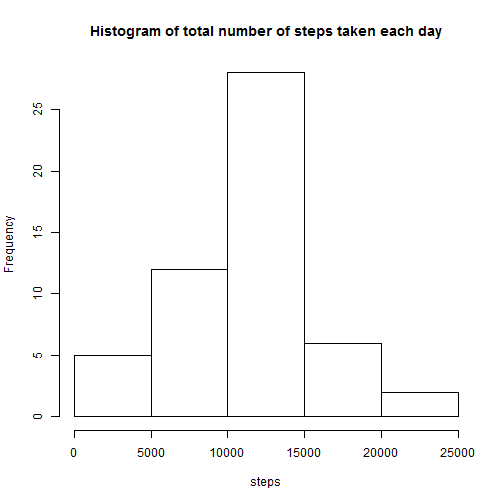
\includegraphics{PA1_template_files/figure-latex/hist-1.pdf}

\begin{Shaded}
\begin{Highlighting}[]
\KeywordTok{mean}\NormalTok{(steps)}
\end{Highlighting}
\end{Shaded}

\begin{verbatim}
## [1] 10766.19
\end{verbatim}

\begin{Shaded}
\begin{Highlighting}[]
\KeywordTok{median}\NormalTok{(steps)}
\end{Highlighting}
\end{Shaded}

\begin{verbatim}
## [1] 10765
\end{verbatim}

\subsection{Calculating average number of steps in each 5-minute
interval, over all
days}\label{calculating-average-number-of-steps-in-each-5-minute-interval-over-all-days}

\begin{Shaded}
\begin{Highlighting}[]
\NormalTok{daily <-}\StringTok{ }\NormalTok{activity %>%}
\StringTok{        }\KeywordTok{filter}\NormalTok{(!}\KeywordTok{is.na}\NormalTok{(steps)) %>%}
\StringTok{        }\KeywordTok{group_by}\NormalTok{(interval) %>%}
\StringTok{        }\KeywordTok{summarize}\NormalTok{(}\DataTypeTok{steps=}\KeywordTok{mean}\NormalTok{(steps)) %>%}
\StringTok{        }\NormalTok{print}
\end{Highlighting}
\end{Shaded}

\begin{verbatim}
## Source: local data frame [288 x 2]
## 
##    interval     steps
##       (int)     (dbl)
## 1         0 1.7169811
## 2         5 0.3396226
## 3        10 0.1320755
## 4        15 0.1509434
## 5        20 0.0754717
## 6        25 2.0943396
## 7        30 0.5283019
## 8        35 0.8679245
## 9        40 0.0000000
## 10       45 1.4716981
## ..      ...       ...
\end{verbatim}

\subsection{Time series plot of the average number of steps in each
5-minute interval, over all
days}\label{time-series-plot-of-the-average-number-of-steps-in-each-5-minute-interval-over-all-days}

\begin{Shaded}
\begin{Highlighting}[]
\KeywordTok{plot}\NormalTok{(daily, }\DataTypeTok{type =} \StringTok{"l"}\NormalTok{)}
\end{Highlighting}
\end{Shaded}

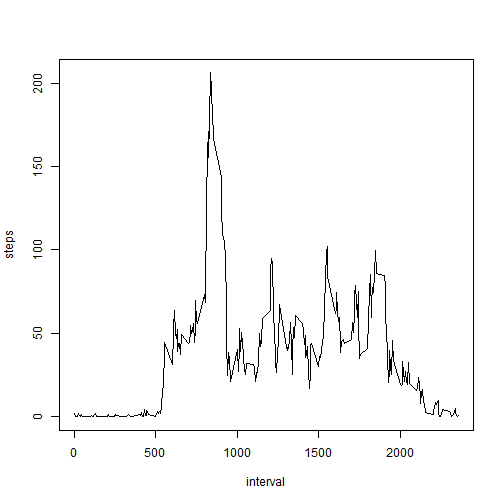
\includegraphics{PA1_template_files/figure-latex/plot-1.pdf}

\subsection{Computing the interval with maximum number of steps,
averaged over all
days.}\label{computing-the-interval-with-maximum-number-of-steps-averaged-over-all-days.}

\begin{Shaded}
\begin{Highlighting}[]
\NormalTok{daily[}\KeywordTok{which.max}\NormalTok{(daily$steps), ]$interval}
\end{Highlighting}
\end{Shaded}

\begin{verbatim}
## [1] 835
\end{verbatim}

\subsection{Reporting the total number of missing values in the
dataset}\label{reporting-the-total-number-of-missing-values-in-the-dataset}

\begin{Shaded}
\begin{Highlighting}[]
\NormalTok{missing <-}\StringTok{ }\KeywordTok{sum}\NormalTok{(}\KeywordTok{is.na}\NormalTok{(activity))}
\NormalTok{missing}
\end{Highlighting}
\end{Shaded}

\begin{verbatim}
## [1] 2304
\end{verbatim}

\subsection{Creating new dataset by filling in missing values with the
mean number of steps for that
day}\label{creating-new-dataset-by-filling-in-missing-values-with-the-mean-number-of-steps-for-that-day}

\begin{Shaded}
\begin{Highlighting}[]
\NormalTok{missing <-}\StringTok{ }\KeywordTok{sum}\NormalTok{(}\KeywordTok{is.na}\NormalTok{(activity))}
\NormalTok{missing}
\end{Highlighting}
\end{Shaded}

\begin{verbatim}
## [1] 2304
\end{verbatim}

\subsection{Computing mean and median of the total number of steps taken
per
day}\label{computing-mean-and-median-of-the-total-number-of-steps-taken-per-day}

\begin{Shaded}
\begin{Highlighting}[]
\NormalTok{new <-}\StringTok{ }\NormalTok{activity %>%}
\StringTok{        }\KeywordTok{group_by}\NormalTok{(interval) %>%}
\StringTok{        }\KeywordTok{mutate}\NormalTok{(}\DataTypeTok{steps =} \KeywordTok{ifelse}\NormalTok{(}\KeywordTok{is.na}\NormalTok{(steps), }\KeywordTok{mean}\NormalTok{(steps, }\DataTypeTok{na.rm=}\OtherTok{TRUE}\NormalTok{), steps))}
\KeywordTok{summary}\NormalTok{(new)}
\end{Highlighting}
\end{Shaded}

\begin{verbatim}
##      steps             date               interval     
##  Min.   :  0.00   Min.   :2012-10-01   Min.   :   0.0  
##  1st Qu.:  0.00   1st Qu.:2012-10-16   1st Qu.: 588.8  
##  Median :  0.00   Median :2012-10-31   Median :1177.5  
##  Mean   : 37.38   Mean   :2012-10-31   Mean   :1177.5  
##  3rd Qu.: 27.00   3rd Qu.:2012-11-15   3rd Qu.:1766.2  
##  Max.   :806.00   Max.   :2012-11-30   Max.   :2355.0
\end{verbatim}

\subsection{Histogram of the total number of steps taken each day, based
on the new
dataset}\label{histogram-of-the-total-number-of-steps-taken-each-day-based-on-the-new-dataset}

\begin{Shaded}
\begin{Highlighting}[]
\NormalTok{new.steps <-}\StringTok{ }\NormalTok{new %>%}
\StringTok{  }\KeywordTok{group_by}\NormalTok{(date) %>%}
\StringTok{  }\KeywordTok{summarize}\NormalTok{(}\DataTypeTok{steps =} \KeywordTok{sum}\NormalTok{(steps)) }
\NormalTok{new_steps <-}\StringTok{ }\NormalTok{new.steps$steps}
\KeywordTok{hist}\NormalTok{(new_steps, }\DataTypeTok{main =} \StringTok{"Histogram of total number of steps taken each day, based on new dataset"}\NormalTok{)}
\end{Highlighting}
\end{Shaded}

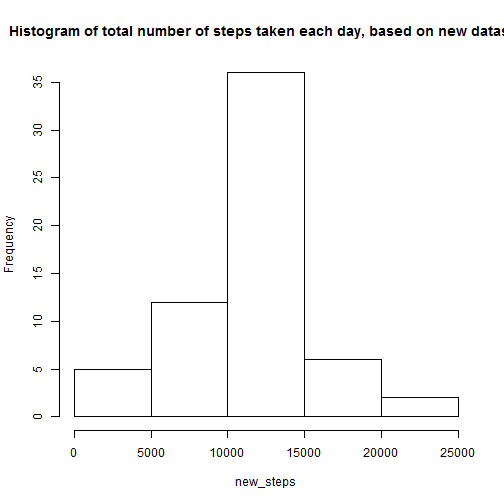
\includegraphics{PA1_template_files/figure-latex/newhist-1.pdf}

\begin{Shaded}
\begin{Highlighting}[]
\KeywordTok{mean}\NormalTok{(new_steps)}
\end{Highlighting}
\end{Shaded}

\begin{verbatim}
## [1] 10766.19
\end{verbatim}

\begin{Shaded}
\begin{Highlighting}[]
\KeywordTok{median}\NormalTok{(new_steps)}
\end{Highlighting}
\end{Shaded}

\begin{verbatim}
## [1] 10766.19
\end{verbatim}

\subsection{Comparing if there is a change in the mean, median values in
the old and new
datasets.}\label{comparing-if-there-is-a-change-in-the-mean-median-values-in-the-old-and-new-datasets.}

\begin{Shaded}
\begin{Highlighting}[]
\KeywordTok{mean}\NormalTok{(steps) ==}\StringTok{ }\KeywordTok{mean}\NormalTok{(new_steps)}
\end{Highlighting}
\end{Shaded}

\begin{verbatim}
## [1] TRUE
\end{verbatim}

\begin{Shaded}
\begin{Highlighting}[]
\KeywordTok{median}\NormalTok{(steps) ==}\StringTok{ }\KeywordTok{median}\NormalTok{(new_steps)}
\end{Highlighting}
\end{Shaded}

\begin{verbatim}
## [1] FALSE
\end{verbatim}

\subsection{Results of comparisom}\label{results-of-comparisom}

Turns out that only the median has shifted.

\subsection{Creating a new factor variable in the dataset, to
distinguish between a ``weekday'' and a
``weekend''.}\label{creating-a-new-factor-variable-in-the-dataset-to-distinguish-between-a-weekday-and-a-weekend.}

\begin{Shaded}
\begin{Highlighting}[]
\NormalTok{dayofweek <-}\StringTok{ }\NormalTok{function(date) \{}
    \NormalTok{if (}\KeywordTok{weekdays}\NormalTok{(}\KeywordTok{as.Date}\NormalTok{(date)) %in%}\StringTok{ }\KeywordTok{c}\NormalTok{(}\StringTok{"Saturday"}\NormalTok{, }\StringTok{"Sunday"}\NormalTok{)) \{}
        \StringTok{"weekend"}
    \NormalTok{\} else \{}
        \StringTok{"weekday"}
    \NormalTok{\}}
\NormalTok{\}}
\NormalTok{new$daytype <-}\StringTok{ }\KeywordTok{as.factor}\NormalTok{(}\KeywordTok{sapply}\NormalTok{(new$date, dayofweek))}
\end{Highlighting}
\end{Shaded}

\subsection{Comparing time plots to find difference in patterns between
weekdays and
weekends}\label{comparing-time-plots-to-find-difference-in-patterns-between-weekdays-and-weekends}

\begin{Shaded}
\begin{Highlighting}[]
\KeywordTok{par}\NormalTok{(}\DataTypeTok{mfrow =} \KeywordTok{c}\NormalTok{(}\DecValTok{2}\NormalTok{, }\DecValTok{1}\NormalTok{))}
\NormalTok{for (type in }\KeywordTok{c}\NormalTok{(}\StringTok{"weekend"}\NormalTok{, }\StringTok{"weekday"}\NormalTok{)) \{}
    \NormalTok{steps.type <-}\StringTok{ }\KeywordTok{aggregate}\NormalTok{(steps ~}\StringTok{ }\NormalTok{interval, }\DataTypeTok{data =} \NormalTok{new, }\DataTypeTok{subset =} \NormalTok{new$daytype ==}\StringTok{ }
\StringTok{        }\NormalTok{type, }\DataTypeTok{FUN =} \NormalTok{mean)}
    \KeywordTok{plot}\NormalTok{(steps.type, }\DataTypeTok{type =} \StringTok{"l"}\NormalTok{, }\DataTypeTok{main =} \NormalTok{type)}
\NormalTok{\}}
\end{Highlighting}
\end{Shaded}

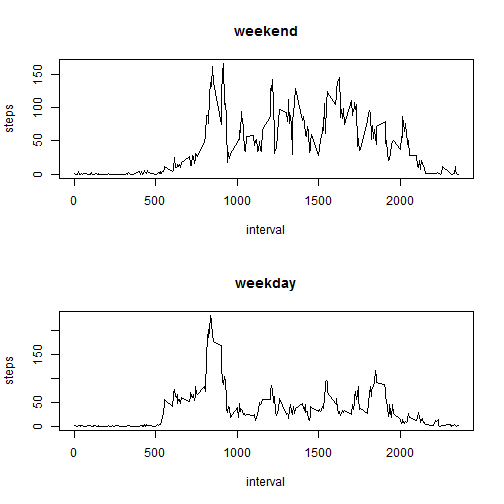
\includegraphics{PA1_template_files/figure-latex/compareplots-1.pdf}

\end{document}
